\subsection{Gate driver}
\begin{figure}[H]
\centering
\fbox{
\begin{circuitikz}[scale = 0.75]
\draw (5,2)
	node[nmos](nmos1) {}
	(nmos1.G) node[right = 10mm]{NTD20N06}
	(nmos1.D) to (5,4)
	(nmos1.S) to (5,0);
\draw (-1,2) to [R, l_=$10 \ \mathsf{\Omega}$] (2,2) -- (nmos1.G);
\draw (2,2) -- (2,1) to [R, l_=$10 \ \mathsf{k\Omega}$] (5,1);
\draw (-1,2) node[ocirc, label=left:PWM] {};
\draw (5,4) node[ocirc, label=above:load] {};
\draw (5,0)	node[ground] {};
\end{circuitikz}
}
\caption{}
% \label{}
\end{figure}
MOSFETs were chosen as the switching component in the SMPS due to its increased power efficiency and rate of switching over a BJT. This increase in switching speed allowed for converter topologies that required smaller inductance and capacitance values, overall leading to smaller component sizes on the board. This was a serious design constraint, as to achieve the desired specifications, considerably large capacitance and inductance values were required. As outlined in section \ref{sec:ss_averaging} component values are inversely proportional to the switching frequency. Hence by choosing a large switching frequency we were able to obtain components that were both small and cost effective.
\\ \\
MOSFETs operate in a fundamentally different way to BJTs, this is in part due to the input impedance of both devices. A MOSFET is a voltage controller current source, and ideally the Gate of the MOSFET has large input impedance resulting in zero current draw. However, in practice the MOSFET gate acts as two separate capacitors, one between gate and drain and the other between gate and source. For the gate voltage to increase, the total input capacitance (sum of both the gate-drain and gate-source parasitic capacitances) must be charged. 
\\ \\
It is important to note that a MOSFET essentially dissipates not power when it either in the fully on or fully of states. The region in between, known as the transition region, is when the transistor dissipates most of its energy. Hence it is important that the time spent in this region in minimized.
\\ \\
%\textbf{discuss the fet that was used}
The output pin of a microcontroller is usually adequate to drive a small-signal logic level MOSFET. However, two issues arise when driving larger power MOSFETs that have been designed to deal with the higher current and voltages of power applications.
\begin{itemize}
    \item Increased gate/input capacitance. Due to the low current sink/source capabilities of microcontrollers, they are designed to only drive relatively small capacitive loads (in the order to 10-100pF). Power MOSFETs on the other hand can have input capacitances on the order of thousands of pico-farads.
    \item Higher gate/threshold voltage. Most power MOSFETs require voltages exceeding \SI{12}{V} to fully turn on. Therefore, a common TTL or CMOS logic signals of \SI{3.3}{V} or \SI{5}{V} is often not enough.
\end{itemize}
To maximize the switching frequency, such that the MOSFET spends the least amount of time in the transition state as possible, we must force a lot of charge into the gate very quickly. This, unsurprisingly, requires large peak currents.
\\ \\
%\textbf{Include calculations of peak gate currents required to attain the high switching speeds.}
%\\ \\
A gate capacitor is included in series with the gate of the transistor. Increasing the resistance resulted in the charging current being reduced, however it also slowed down the maximum switching speed. Reducing the current flow in the gate too much resulted in the gate charging slower than the speed it was switched, producing significant distortion of the waveform. 
\\ \\
Decreasing the gate resistor $R_g$ resulted in faster switching, however this produced larger current spikes in excess of $\pm\SI{300}{mA}$. This was simulated in LTSpice with the chosen MOSFET’s SPICE model.
\begin{itemize}
    \item Rise/fall time of a PWM signal produced by the MCU PWM module was minimum 5ns.
    \item \SI{10}{\ohm} have an appropriate response while limiting the instantaneous current, however it was still upwards of $\pm\SI{200}{mA}$.
    \item PWM frequency of \SI{250}{kHz}. Chosen to allow for flexibility in the design of the \'Cuk converter.
\end{itemize}
\SI{420}{\ohm} limits the gate current to under \SI{12}{mA} however this significantly distorted the PWM signal as the MOSFET is no longer driven to saturation during the switch on time. Hence a gate driver IC is required. See simulation results in \textbf{appendix ??} for detailed analysis. 
\\ \\
The Microchip TC4427A was chosen as the gate driver for the hardware implementation. It was chosen due to a number of features:
\begin{itemize}
    \item Non-inverting output meant that the control algorithm implemented on the microcontroller didn’t need to be altered in order for it to operate correctly.
    \item Wide Input Supply Voltage Operating Range (\SI{4.5}{V} to \SI{18}{V}). Allowed for a wide range of MOSFETs to be driven with the same chip.
    \item High Capacitive Load Drive Capability (\SI{1000}{pF}) and High Peak Output Current (\SI{1.5}{A}).
\end{itemize}
Finally, the TC4427A was included in the LTSpice model and produced an identical response. However, it can safely source and sink the required current. See appendix \ref{apx:sim_mosfet}.
\begin{figure}[H]
    \centering
    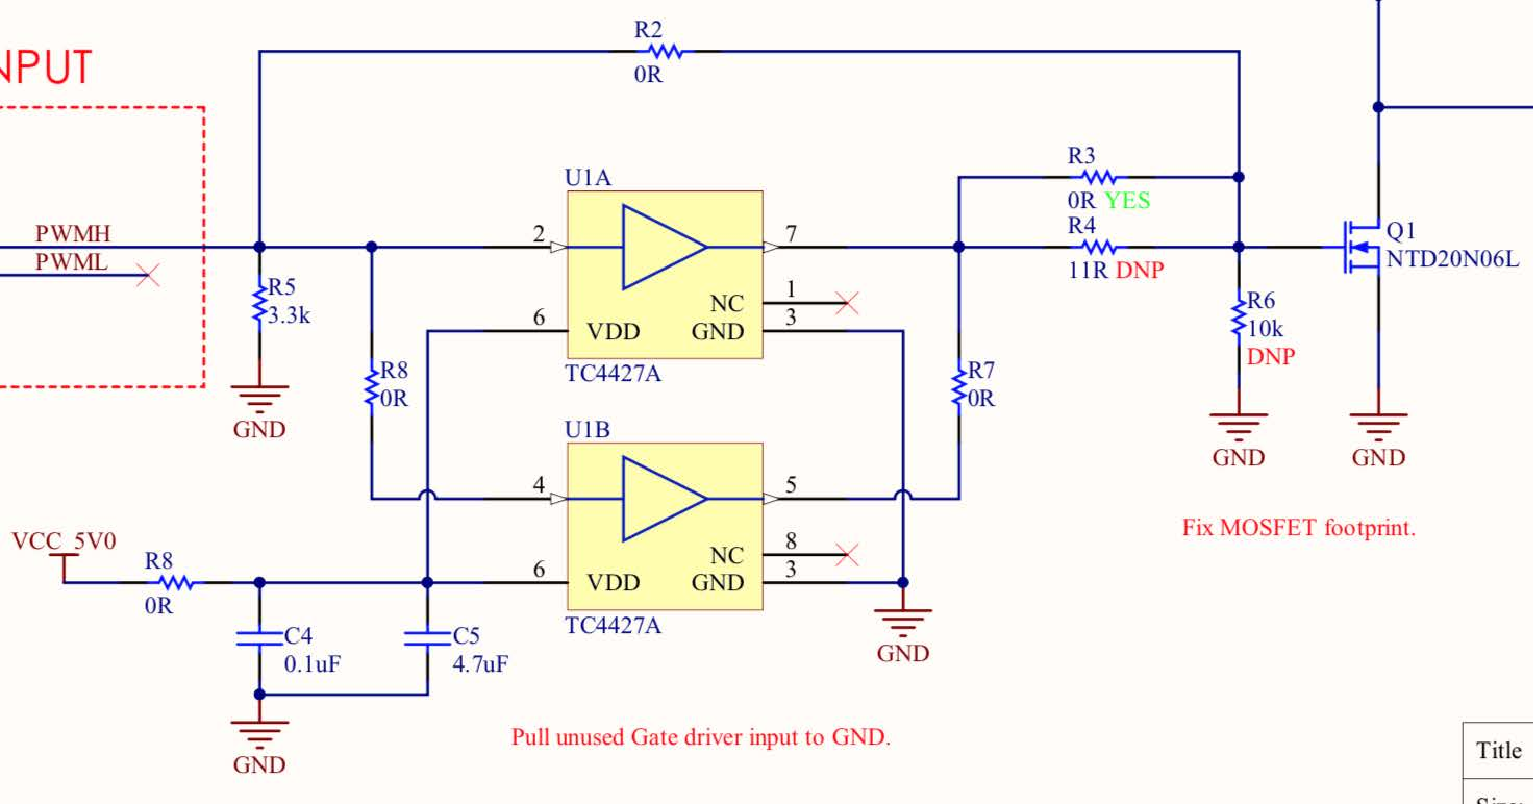
\includegraphics[height = 8cm]{figures/hardware/gate_driver_schematic.pdf}
    \caption{Gate driver schematic excerpt.}
    \label{fig:gate_driver}
\end{figure}